% Beamer template
% Author: Ozgur Taylan TURAN
% Delft University of Technology

\documentclass[aspectratio=169]{beamer}
% PACKAGES
\usepackage[english]{babel}
\usepackage{graphicx}
\usepackage{animate}
%\usepackage{calc}
\usepackage{calligra}
\usepackage[absolute,overlay]{textpos}
\usepackage[T1]{fontenc}
%\usefonttheme{serif}
\usefonttheme{professionalfonts}
\usepackage{amsmath}
\usepackage{palatino}
\usepackage{mathpazo}
\usepackage{graphicx}
%\usepackage{subfig}
\usepackage{tikz}
\usetikzlibrary{shapes,arrows}
\usepackage{xcolor}
\usepackage[T1]{fontenc}
%\usefonttheme{serif}
%\usepackage{titling}
\usepackage{graphicx}
%\usepackage{subfig}
%\usepackage{tikz}
%\usetikzlibrary{shapes,arrows}
\usepackage{mathtools}
\usepackage{cancel}
% CUSTOM PACKAGES
\usepackage{/home/taylanot/texmf/tex/beamerthemetot}
\input{/home/taylanot/texmf/presentation/tune.tex}

 % COVER PAGE INFO   
\newcommand{\mytitle}{\color{White}\huge{\textbf{Meta-Learning \#3}}}
\newcommand{\mysubtitle}{\color{Pink}\Large{\textbf{Generalization of MAML for Linear Problems}}}
\newcommand{\myauthor}{\color{White}\textcalligra{\LARGE Ozgur Taylan Turan}}
\newcommand{\authorlabel}{\small O.T. Turan}
\author{\authorlabel}


\begin{document}
% COVER PAGE

{
\def\beamer@entrycode{\vspace*{-\headheight}}
\setbeamertemplate{frametitle}[default][center]
\setbeamertemplate{navigation symbols}{}
\usebackgroundtemplate{
\includegraphics[width=\paperwidth,height=\paperheight]{cover/coverart.pdf}}

\begin{frame}[plain] 

\begin{minipage}{\textwidth}
	\centering{\mytitle} \\
	%\vspace{1cm}
	%\centering{\mysubtitle} \\
	\vspace{1cm}
	\centering{\color{White}November 15, 2021} \\
	\vspace{1cm}
	\centering{\myauthor}\\
\end{minipage}
\end{frame}
}


\begin{frame}
	\centering
	\mysubtitle
\end{frame}

\section{Problem}
\begin{frame}{Problem}
  \centering
   $y = \mathbf{x}\mathbf{a}^\text{T} + \underbrace{\varepsilon}_{\mathcal{N}(0,\sigma=1)}$
  \begin{itemize}
    \item $\mathbf{a}\in\mathbb{R}^D$ represents the task
    \item Assume $\mathbf{a}\sim\mathcal{N}(m\boldsymbol{1},c\boldsymbol{I})$, where $\boldsymbol{1}\in\mathbb{R}^{D\times 1}$ and $\boldsymbol{I}\in\mathbb{R}^{D\times D}$
    \item Training data $Z:=(\mathbf{x}_i,y_i)_{i=1}^{N}$ are drawn from distribution distribution $p_Z$.
    \item $p_x \sim \mathcal{N}(\boldsymbol{0},k\boldsymbol{I})$
    \item Expected Loss is  $\mathcal{E}:=\large\iiint(\mathbf{x}\hat{\mathbf{a}}_N(Z)^\text{T}-y)^2p(\mathbf{x},y)d\mathbf{x}dyp_ZdZp_\mathbf{a}d\mathbf{a}$.
  \end{itemize}
\end{frame}

\section{Models}
\begin{frame}{Models}
  \centering
  $\mathcal{M}(\mathbf{w,b,\mathbf{x}}):= \mathbf{w}^\text{T}\mathbf{x}+b$ \\

  $\mathcal{L}:=||\mathbf{y}-\mathcal{M}(\bar{\mathbf{w}}, \mathbf{X})||^2$ \\ 

  $\mathcal{L}_{\text{ridge}}:=||\mathbf{y}-\mathcal{M}(\bar{\mathbf{w}}, \mathbf{X})||^2+\lambda||\bar{\mathbf{w}}||^2$ \\

  $\mathcal{L}_{\text{gen.ridge}}:=||\mathbf{y}-\mathcal{M}(\bar{\mathbf{w}}, \mathbf{X})||^2+\lambda||\bar{\mathbf{w}}-\mathbf{h}||^2$ \\
  \only<1>
{
  \begin{block}{\color{White} Note that,}
    \begin{itemize}
      \centering
      \item $\mathbf{X}=\begin{bmatrix}\mathbf{x}_1& 1\\ \vdots & \vdots \\ \mathbf{x}_n& 1\end{bmatrix}_{N\times(d+1)}$ , $\quad\bar{\mathbf{w}}=\begin{bmatrix}\mathbf{w}\\ {b}\end{bmatrix}_{(d+1)}$ and  $\mathbf{h}\in\mathbb{R}^{D\times 1}$
    \end{itemize}
  \end{block}
}
\only<2>
{
  \begin{itemize}
    \item Linear:  $\bar{\mathbf{w}}=(\mathbf{X}^{\text{T}}\mathbf{X})^{-1}\mathbf{X}^{\text{T}}\mathbf{y}$
    \item Ridge:  $\bar{\mathbf{w}}=(\mathbf{X}^{\text{T}}\mathbf{X}+\lambda\mathbf{I})^{-1}\mathbf{X}^{\text{T}}\mathbf{y}$
    \item GeneralRidge\cite{Denevi2018a}:  $\bar{\mathbf{w}}=(\mathbf{X}^{\text{T}}\mathbf{X}+\lambda\mathbf{I})^{-1}(\mathbf{X}^{\text{T}}\mathbf{y}+\lambda\mathbf{h})$
    \item GD: $\mathbf{w}_{niter+1}=\mathbf{w}_{niter}-l_r*\frac{2}{N}\sum_{i=1}^{N}\mathbf{x}_i\big((\mathbf{w}_{niter}^{\text{T}}\mathbf{x}_i+b)-y_i\big)$ and $b_{niter+1}=b_{niter}-l_r*\frac{2}{N}\sum_{i=1}^{N}\big((\mathbf{w}_{niter}^{\text{T}}\mathbf{x}_i+b)-y_i\big)$
  \end{itemize}
}
\end{frame}

\begin{frame}{Additional Info}
  \begin{itemize}
    \item GD: starts from $\bar{\mathbf{w}}_{\text{opt}}$ and takes step with drawn training samples
    \item MAML: start GD from $\bar{\mathbf{w}}\sim\mathcal{N}(\bar{\mathbf{w}}_{\text{opt}},0.1\mathbf{I})$
    \item randomGD: start with a random initialization for $\bar{\mathbf{w}}$
    \item Bayes: Bayes error resulting from the $\bar{\mathbf{w}}_{\text{opt}}$
  \end{itemize}
\end{frame}

\section{Aim}
\begin{frame}{Aim}
  \begin{itemize}
    \item See the effect of the MAML adaptation.
    \item See if Ridge Regression can compete with a task informed algorithm.
  \end{itemize}
\end{frame}

\begin{frame}{Experiments}
  \begin{itemize}
		\item $n_{iter}:[0,90;10]$, $\sigma:[0,5;50]$, $D:[1,50;50]$, $m:[0,10;50]$, $c:[0,10,50]$, $b:[1,5,50]$, $N:[1,10;50]$
	\item $\lambda:[0.0001,20;10]$, $l_r:[0.0001,1,10]$
	\item  $N_{test}:1000$, $N_{a}:100$, $N_{Z}:100$, $m=0$, $c=1$, $\sigma=1$
  \end{itemize}
\end{frame}
\section{Results}
\begin{frame}{Task Variance($c$)}
\only<1>
{
\centering
  \color{Pink} Increasing $N:1\to 10 \to 50$ and $D:1$
  \begin{minipage}{0.33\textwidth}
    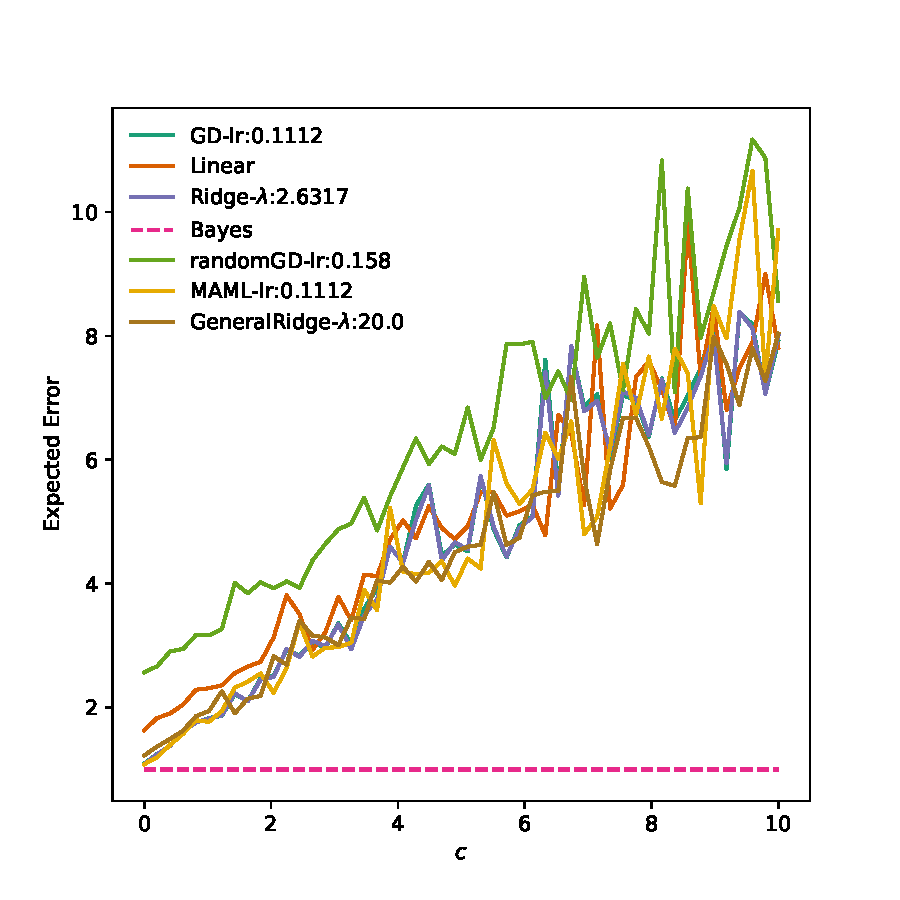
\includegraphics[width=\textwidth]{Figures/c-1-1-x-0.pdf}
  \end{minipage}%
  \begin{minipage}{0.33\textwidth}
    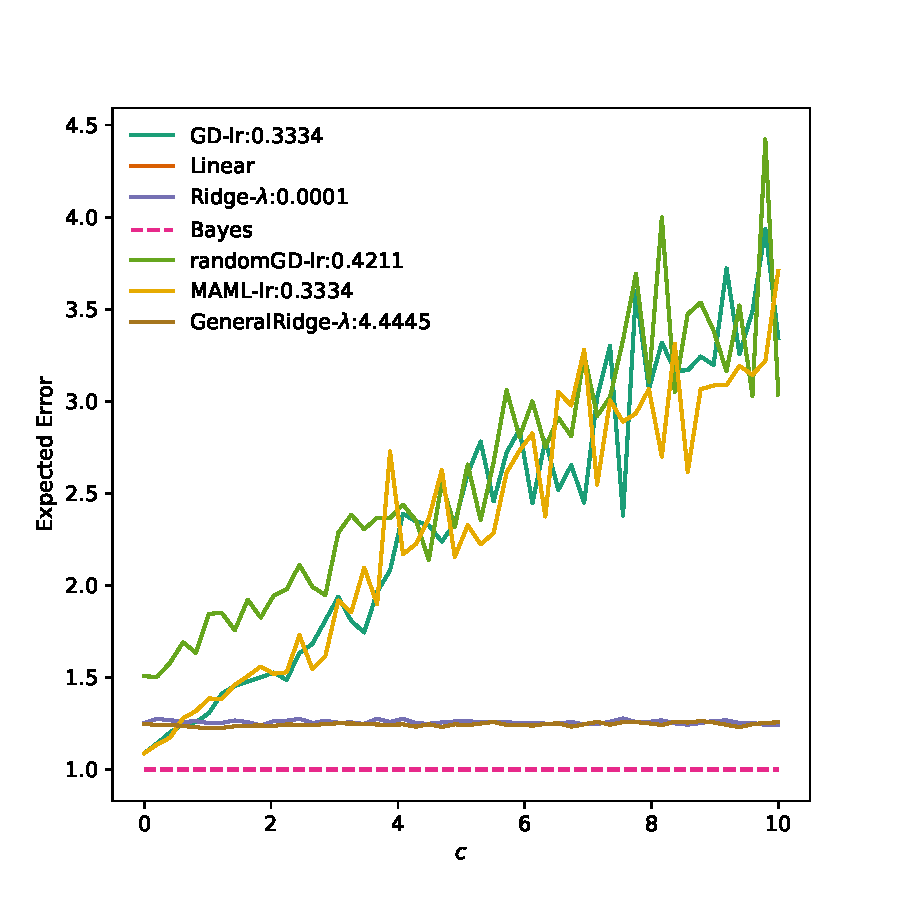
\includegraphics[width=\textwidth]{Figures/c-1-10-x-0.pdf}
  \end{minipage}%
  \begin{minipage}{0.33\textwidth}
    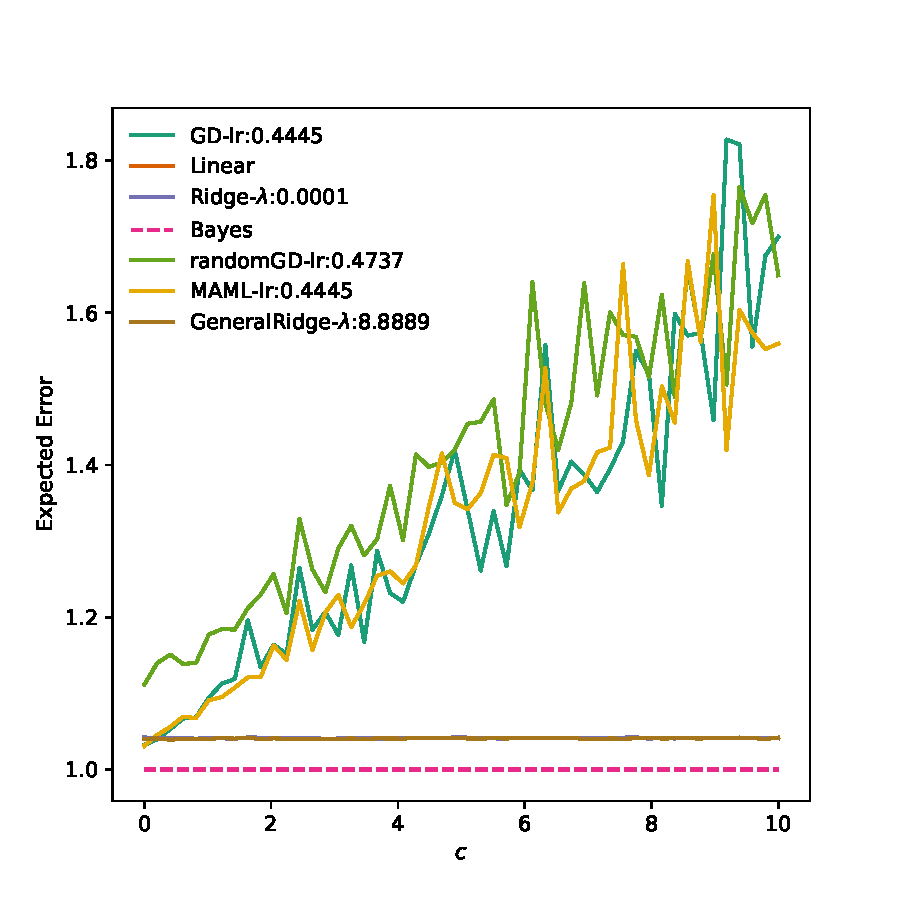
\includegraphics[width=\textwidth]{Figures/c-1-50-x-0.pdf}
  \end{minipage}
}
\only<2>
{
\centering
  \color{Pink} Increasing $D:1\to 10 \to 50$ and $N:10$
  \begin{minipage}{0.33\textwidth}
    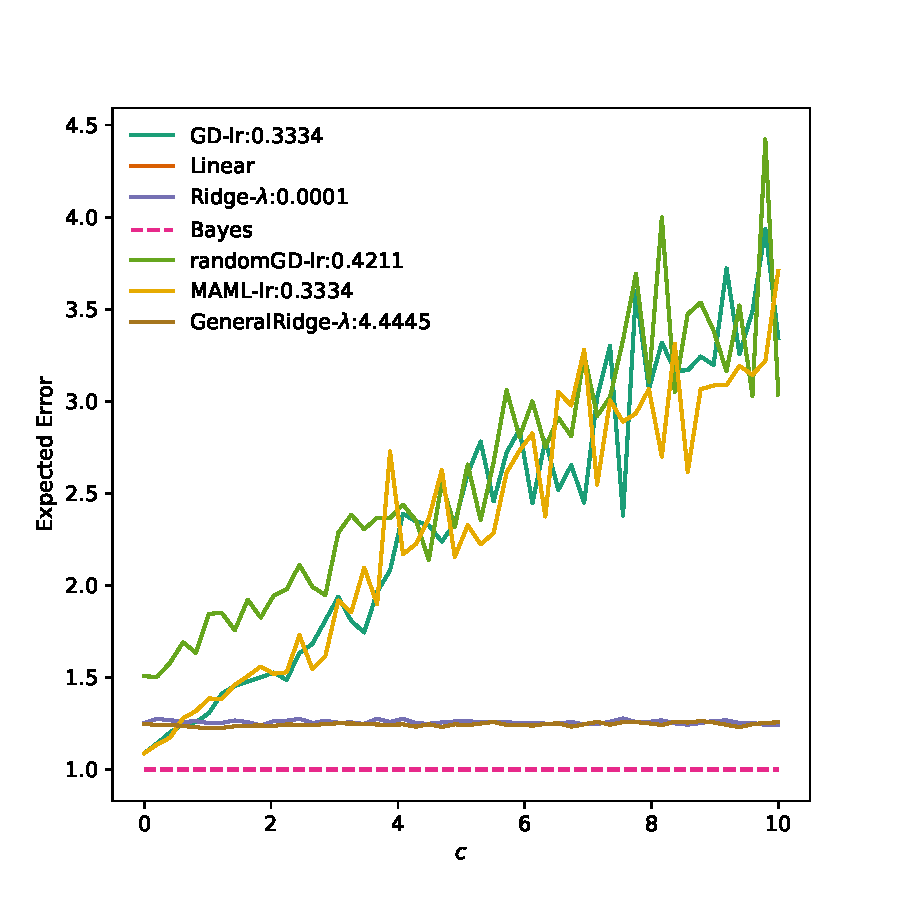
\includegraphics[width=\textwidth]{Figures/c-1-10-x-0.pdf}
  \end{minipage}%
  \begin{minipage}{0.33\textwidth}
    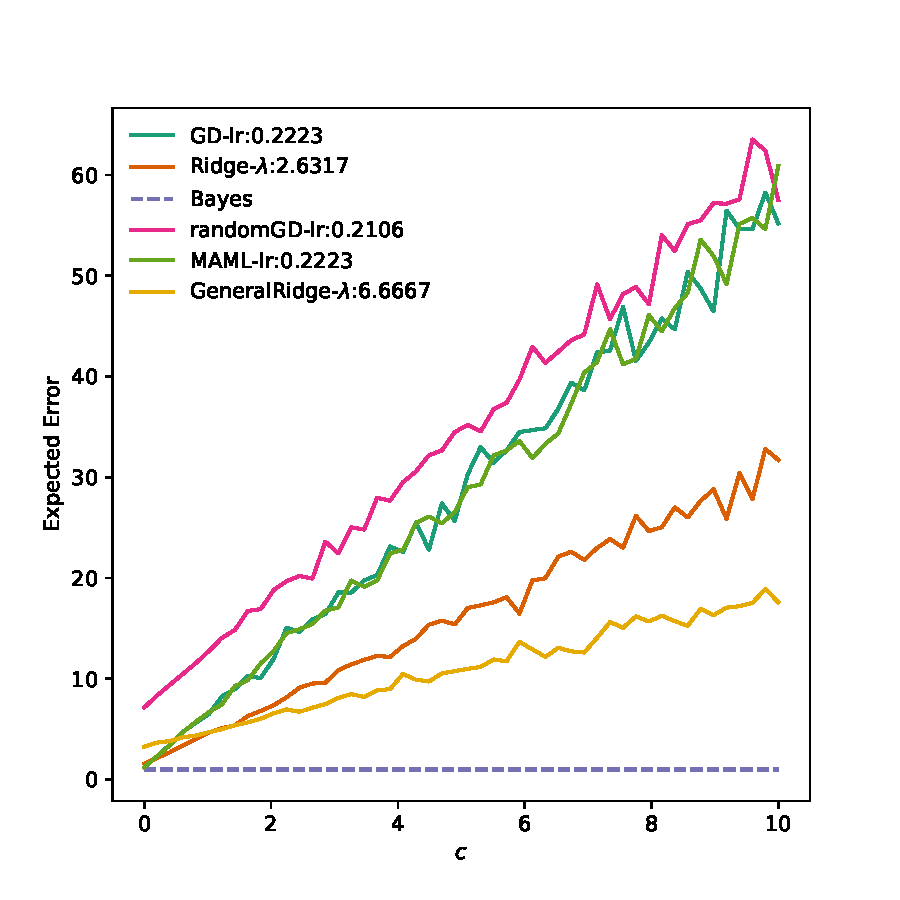
\includegraphics[width=\textwidth]{Figures/c-10-10-x-1.pdf}
  \end{minipage}%
  \begin{minipage}{0.33\textwidth}
    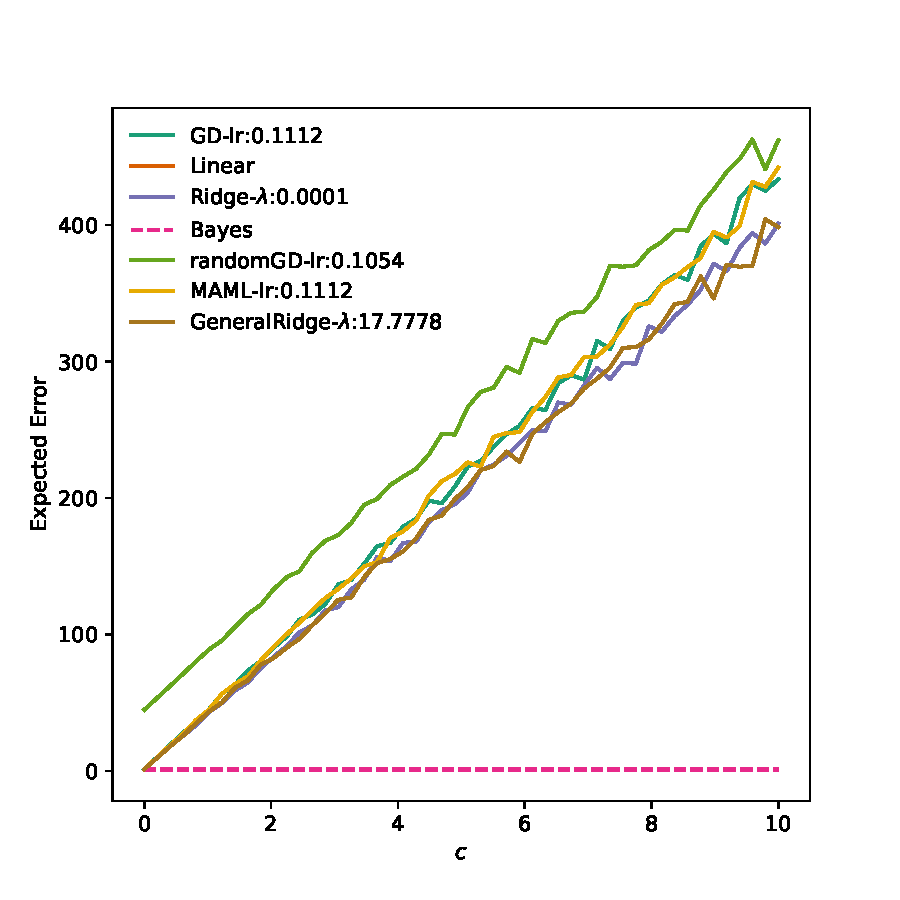
\includegraphics[width=\textwidth]{Figures/c-50-10-x-0.pdf}
  \end{minipage}
}
\end{frame}

\section{Coming Up}
\begin{frame}{Next}
  \begin{itemize}
    \item Investigation of that little area where the MAML performs better only over all the experimentation. Increasing dimensions. (Fresh out results!)
    \item Writing the Draft! (Started!)
    \item Non-linear experimentations (Next-week!) [Predicting the sine-wave with changing amplitude and the phase...] 
  \end{itemize}
\end{frame}

\section{Struggles}
\begin{frame}{Struggles}
  \begin{itemize}
    \item Kernel Ridge for GeneralRidge like bias parameter?
    \item Why is it not common to gradient descent with Kernel Ridge regression?
  \end{itemize}
\end{frame}

\end{document}
